\chapter{引言}
\section{钛工业的发展历程与国内外现状}

钛(Titanium),原子序数为22,最早于1791年由格雷戈尔在英国康沃尔郡发现,是一种银白色的金属,具有密度小、比强度高、耐高温、化学性质性质稳定等明显优于传统金属的特性而备受重视。钛及钛合金常用来制造飞机、火箭等航天机械,一直以来都是航空航天工业的“脊柱”之一,被誉为“太空机械”\cite{XJYS200102014}。与纯钛一同发展起来的钛合金也毫不逊色,钛合金是在纯钛的基础上添加了各种各样的合金元素而形成的合金,凭借其更高的强度、耐蚀性、抗高温性能,得到了广泛的应用,尤其是在机械制造、航空航天、化工、军工等领域,钛合金的占比更大。钛工业的发展水平在一定程度上是衡量一个国家航空航天、汽车工业等发展水平的重要标志\cite{HSJJ202109005}。

\subsection{钛与钛合金的特点}
钛合金具有密度小,强度高的显著特点,相较于高强度钢而言,不仅强度相差无几,而且还具有更大的比强度。

\begin{table}[htbp]
	\centering
	\label{sec:bqd}
	\caption{不同合金比强度比较表}
	\begin{tabular}{ccccc}
		\toprule
		\textbf{合金} & \textbf{镁合金} & \textbf{铝合金} & \textbf{高强钢} & \textbf{钛合金} \\
		\midrule
		比强度 & 16 & 21 & 23 & 29 \\
		\bottomrule
	\end{tabular}
\end{table}

钛合金的特点如下\cite{1997titanium}:
\begin{enumerate}
	\item 熔点高,钛的熔点为1668℃,比铁的熔点还高出138℃。加入合金元素后可以获得极佳的热强性。
	\item 弹性模量低,屈服强度高,适合做弹簧材料,高端赛车内部的弹簧大多数都是由钛合金制成,它同时还具有较好的耐磨性。
	\item 表面极易生成致密的氧化层,在氧化性或中性介质中有较强的耐腐蚀能力。
	\item 此外还有无磁性,,形状记忆性等优良特点。
	\item 化学活性高,当钛加热到500℃以上时,氧化膜变得稀松且易脱落,在熔融状态下,极易发生自然。
	\item 此外,某些钛合金还具有储氢、超导、低阻尼性,生物相容性、形状记忆 、 超弹 、高阻尼等特殊功能。
\end{enumerate}

由于钛合金具有以上诸多特点,目前已广泛应用于自动化 、能源 、航空航天 、 医	疗卫生 、 汽车和家电等领域。
\subsection{国外发展}
钛工业的发展充满曲折。从钛元素的发现(1791)到第一次制得较纯的金属钛(1910)经历了120年的历程。又由实验室第一次获得纯钛(1940)到首次进行工业生产,又花费了近30年的时间。
钛在自然界中主要以钛矿石的形式存在,如钛铁矿、金红石(TiO2)等,需要进行精炼(refining)才能获得纯金属。起初,钛的提取是通过高温还原法,但这种方法费时费力,成本高昂。直到了二十世纪四十年代,一种利用氯化钛矿与氯气进行反应来制备四氯化钛,然后通过还原反应(比如Na、Mg等)来得到纯钛的精炼工艺方法终于以其低廉的成本、高效的回收率得到了广泛的商业化应用。

第二次世界大战之后,世界上许多国家都开始意识到钛工业的重要性,钛工业在数年间便迅速发展成为航空、航天、军事等领域的关键材料。1954年,美国成功研发出一种Ti-6Al-4V合金,这种合金在耐热性、强度、塑性、韧性、成形性、可焊性、耐蚀性和生物相容性方面均达到较高水平,使它成为钛工业的主要合金,并占据全部用钛量的50%以上,可以说,许多其他型号钛合金也可以作为Ti-6Al-4V的改良版\cite{COLO200102000}。

\subsection{国内发展}
我国的钛工业发展起源于20世纪50年代,在六七十年代,成为了世界上第四个拥有完整钛工业体系的国家。自21世纪以来我国钛工业进入高速发展阶段,产能与产量已经连续多年占据世界第一的位置,目前海绵钛产量占全球比重已经达到六成,钛加工材产量稳定增长,钛产品消费端需求旺盛\cite{JSTB202209001},无论是在生产还是在加工领域均保持在世界前列,我国已成为名副其实的世界钛工业大国。2014年,浙江余杭高端钛材的研发投产,标志着中国彻底摆脱了对国外的依赖,填补了中国高端钛材的技术空白。\cite{TGYJ200405004}

目前,我国的钛产品消费正处于上升期,如工业、航空航天、海洋船舶和体育休闲等中高端领域的钛材料的需求量平均增长约20%,而医疗行业受疫情影响,需求有所减少,电力和制盐等行业仍有小幅增长,整体盈利水平也有所改善\cite{BJKY202204004}。

此外,近年来计算机技术的发展也为钛工业带来了新的发展机遇。计算机模拟技术用于优化钛合金的生产工艺,显著提高了产品质量。邵一涛等通过采用BP人工神经网络方法建立TC17钛合金组织与性能的关系模型,克服了传统BP人工神经网络训练高精度而预测低精度的过拟合问题\cite{BP};计算机辅助设计和制造技术也为钛制品的设计和生产带来了更多的可能,李淼泉等人对 TC6 合金叶片在等温锻造过程中初生α晶粒尺寸的演变进行了数值模拟\cite{Moni},将有限元法与 Yada 微观组织模型结合起来,并给出了 TC6 合金叶片在等温锻造过程中初生α相的分布和晶粒尺寸的变化。在未来,随着物联网、大数据、人工智能、AIGC等技术的不断发展,钛工业也将迎来更多新的机遇和挑战。
\subsection{应用领域}

进入21 世纪以来,钛工业在多个领域遍地开花。
\begin{itemize}
	\item 	在航空航天领域中,大型客机的研制如火如荼、军机也处于过渡时期,世界航空工业对钛合金的需求也随之迅猛增长。
	\item 在医疗健康领域,由于钛合金生物相容性良好,可以降低人体对植入物的排斥反应和感染风险,它也被广泛用于制造人工关节、牙科种植体和其他医疗设备。
	\item 在汽车制造领域,钛合金的应用主要集中在高档汽车的制造中。钛合金零部件可以减少车辆的自重,从而提高燃油效率和运行性能。同时,钛合金也具有优异的耐腐蚀性能,可以延长汽车零部件的使用寿命。
	\item 在建筑工程领域,钛合金被广泛应用于大型建筑的外墙幕墙、顶棚和立面系统。钛合金具有良好的耐候性和抗腐蚀性能,可以抵御各种恶劣气候条件的侵蚀,并且具有高度的可塑性和装饰性,可以为建筑带来更加优美的外观。

\end{itemize}
\section{钛合金的分类}
\label{sec:1.1}
由于纯钛的强度很低,限制了其在工业生产中的应用。为了满足实际生产中高强度、耐腐蚀性等要求,可以向纯钛中添加一些合金元素形成钛合金。
\subsection*{合金元素}
工业钛合金的主要合金元素为铝、钒、钼三种,此外还有Cr、Mn、Fe、Cu、Sn、Zr、W等元素组成,可以根据合金元素对钛多晶型转变温度的影响可将其分为三大类:$\alpha$稳定元素、$\beta$ 稳定元素、中性元素,形成的四种类型的相图示意图如图1.1所示。
\begin{figure}[h!]
	\centering
	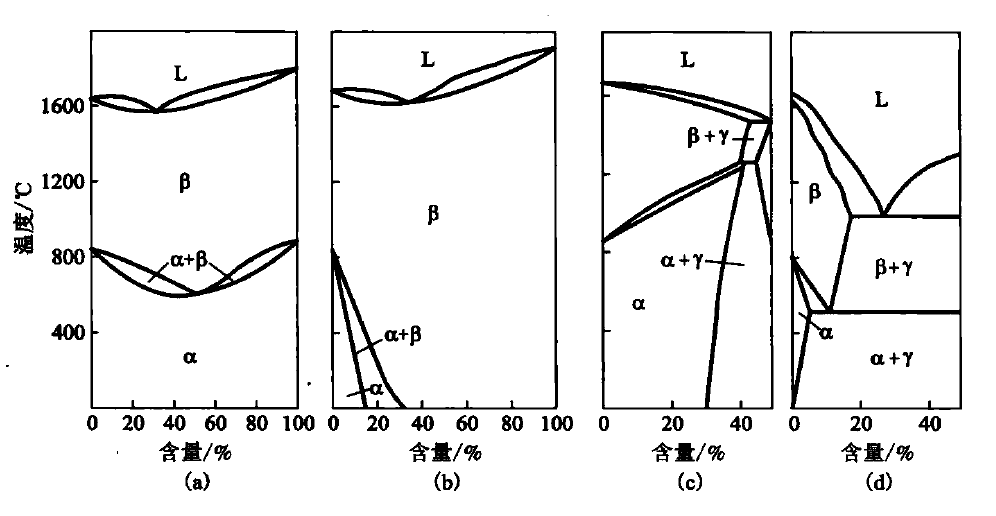
\includegraphics[width=0.9\linewidth]{pic/01}
	\caption{合金元素对钛合金相图的影响示意图}
	\label{fig:01}
\end{figure}

工业上一般根据β相稳定元素系数$K_{\beta}$来划分不同的合金元素,$K_{\beta}$是指合金中各β稳定元素与各自的临界浓度的比制之和,即:
$$
K_{\beta}=\frac{ C_{1} }{C_{k1}}+\frac{ C_{2} }{C_{k2}}+\frac{ C_{3} }{C_{k3}}+\cdots+\frac{ C_{n} }{C_{kn}}
$$
根据 $\beta$ 相稳定系数划分合金类型为:
\begin{enumerate}
	\item  $\alpha$ 型合金 $K_\beta$ 为 $0 \sim 0.07$
	\item 近 $\alpha$ 型合金 $K_\beta$ 为 $0.07 \sim 0.25$
	\item $\alpha+\beta$ 型合金 $K_\beta$ 为 $0.25 \sim 1.0$
	\item 近 $\beta$ 型合金 $K_\beta$ 为 $1.0 \sim 2.8$
	\item $\beta$ 型 合金 $K_\beta$ 为 > 2.8
\end{enumerate}
\subsection*{(1)α型}
α型钛合金经退火处理,其组织常以单相的α固溶体或者以含微量金属化合物的α固溶体形式存在,主要合金元素为铝、锡、锆等α稳定元素,并少量含有钒、 钼、铌等中性元素,各个元素均可起到固溶强化的作用。

常用的α型钛合金包括TA1、TA2、TA7等。

α型钛合金的β相转变温度较高,因而具有良好的热强性、高温稳定性。焊接性性能好,并在高温环境下具有极好的组织稳定性和抗蠕变性能,在低温环境下也依然保持良好的延展性,因而适合制作各种飞行器形状复杂的外层板材。但它对热处理和组织类型不敏感,故不能采用热处理的方式强化其组织\cite{TiandAl}。
\subsection*{(2)β型}
β型钛合金中主要有钒、钼、铌、钽等β相稳定元素,若在合金中加入少量的 铝、锆、锡,可提高β型钛合金的塑性并改善其热稳定性。

常见的β型钛合金有TB1~TB5、TB7、TB10等。

β型钛合金的显微组织 一般比α型、α+β型钛合金的显微组织更粗大。β型钛合金常表现出良好的冷成形、冷加工性能,较好的淬火态塑性以及可焊接性,但是亚稳态β型钛合金热稳定性 较差β型钛合金含有较高的β稳定元素,主要分为稳定β型钛合金和亚稳定β型钛合金。稳定β型钛合金在平衡状态下全部由稳定的β相,热处理后不易产生变化。
\subsection*{(3)α+β型}
α+β型钛合金经退火处理,所得到的室温组织为不同比例的α和β相。该类型的钛合金中除含有定量的铝元素外,还含有少量的其它元素。可采用适当的热处理方法对α+β型钛合金进行组织强化,α+β型钛合金的强度和淬透性随着β相稳定元素含量增加而提高,其锻造和轧制等加工成型性能优于α型、β型钛合金。

最常用的α+β型钛合金包括TC4、TC6、TC12等,其中TC4钛合金(等轴马氏体型两相合金)作为做早被应用的钛合金,该合金以其优越的性能占据了钛工业的大量市场,现在占到 Ti 合金总产量的 50$ \%  $, 占到全部Ti 合金加工件的95$ \% $ 。

从成分上来看,这类钛合金中的合金元素基本上是以铝为主要合金元素,β稳定化元素为辅助元素。这使得α+β型钛合金组织变动的余地较为灵活,性能变动范围大,可以满足各种应用场合及工况要求\cite{TiandAl}。
\section{钛合金的显微组织}
众所周知,材料的最终性能是由显微组织的形态决定的, 不同的组织对应于不同的力学性能, 而微观组织形态主要取决于合金的化学成分、变形工艺和热处理方式等。

前面提到过:钛合金的基本组织是由密排六方的低温 $\alpha$ 相和体心立方的高温 $\beta$ 相构成。 而且除了少数稳定 $\beta$ 型钛合金之外, 体心立方的高温 $\beta$ 相一般都无法保留到室温, 冷却过程中会发生 $\beta$ 相向 $\alpha$ 相的多晶转变, 以片状形态从原始 $\beta$ 晶界析出。片状组织由片状 $\alpha$ 与片状 $\alpha$ 之间的残余 $\beta$ 相构成, 由于其与母相之间存在着一定的结晶 学位向关系, 称为 $\beta$ 转变组织。片状组织在 $\alpha+\beta$ 两相区承受足够大的塑性变形 后再结晶球化得到等轴组织。因此, 按照晶内 $\alpha$ 相的形状变化, $\alpha+\beta$ 型钓合金 的显微组织大致分为 4 类:

\begin{itemize}
	\item 	\textbf{等轴组织}:在 $\beta$ 转变温度以下 $30 \sim 100{ }^{\circ} \mathrm{C}$ 加热, 经过充分的塑性变形和再结晶退火形成。具有较好的塑性,延伸率和较高的断面收縮率,且抗缺口敏感性和热稳定性最好。综合性能好,使用广泛。
	\item 	\textbf{网篮组织}:在 $\beta$ 区加热或开始变形, 在 $\alpha+\beta$ 两相区的变形量不太大时形成。具有高的持久强度和蠕变强度,在热强性方面具有明显的优势,具有高的断裂韧性、低的疲劳裂纹扩展速率。缺点是塑性和热稳定性较低。
	\item 	\textbf{双态组织}:在 $\alpha+\beta$ 两相区的上部加热或者进行变形可以获得。双态组织兼顾了等轴组织和片状组织的优点, 等轴 $\alpha$ 含量在 $20 \%$ 左右的双态组织具有强度 - 塑性 - 韧性 - 热强性的最佳综合匹配。与片状组织相比, 双态组织具有更高的屈服强度、塑性、热稳定 性和疲劳强度; 与等轴组织相比, 双态组织具有较高的持久强度、蜻变强度和断 裂韧性, 以及较低的疲劳裂纹扩展速率 $\mathrm{d} a / \mathrm{d} N$ 。
	\item 	\textbf{魏氏组织}:在较高温度的 $\beta$ 区加热或变形量不够,时可以形成。魏氏组织具有最高的蠕变抗力、持久强度和断裂韧性, 但是其致命的弱点是塑性低, 尤其是断面收缩率远低于其他组织类型。类似于钢中的过热组织, 在实际生产过程中没有特殊的需求应尽量避免。
\end{itemize}

\begin{table}[htbp]
	\centering
	\label{sec:detial}
	\caption{不同组织的性能}
	\begin{tabular}{ccccc}
		\toprule
		机械性能 & 抗拉强度 $ \sigma$ MPa & 延伸率 $\delta\%$ & 冲击韧性& 断裂韧性 \\  \midrule
		片层组织 & 1020 & 9.5 & 355.3 & 102 \\
		网篮组织 & 1010 & 13. 5 & 533 & - \\
		双态组织 & 980 & 13 & 434.3 & - \\
		等轴组织 & 961 & 16.5 & 473.8 & 58.9 \\ \bottomrule
	\end{tabular}
\end{table}
\section{钛合金的相变}
钛合金中的相变主要包括:多晶转变、共析转变、有序化、亚稳相等稳转变、非等温转变等。

%	众多研究者已将钛合金的相变类型绘制成了一个表格:
%	\begin{table}[htbp]
	%	\centering
	%	\label{sec:change}
	%	\caption{相变过程}
	%		\begin{tabular}{ccc}
		%			\hline
		%			编号 & 相变 & 过程 \\ \hline
		%			I & 淬火过程中$\beta$相的分解 & (1)钛的马氏体:$ \beta $ 	o $\alpha^{'}$ , $\alpha^{"}$\$ \\ \hline
		%	~ & 淬火过程中$\beta$相的分解 & (2)无热\$$\backslash$omega\$相:\$$\backslash$beta $\backslash$to $\backslash$omega\_\{$\backslash$text\{无热}} +$\backslash$beta\$ \\ \hline
%II & 等温转变中$\beta$相的分解 & (1) \$$\backslash$beta($\backslash$beta+$\backslash$alpha)$\backslash$to a\^\{"},a\^\{"}$\backslash$text\{富},a\^\{"}$\backslash$text\{贫}\$ \\ \hline`
%~ & 等温转变中$\beta$相的分解 & (2) \$$\backslash$beta\^\{'}$\backslash$beta$\backslash$text\{富},$\backslash$beta$\backslash$text\{贫}\$ \\ \hline
%III & 残余$\beta$相分解 & (1)      相离析: \$$\backslash$beta\_\{$\backslash$text\{残}} $\backslash$to $\backslash$beta\^\{'}+$\backslash$beta\$ \\ \hline
%\end{tabular}
%\end{table}

由于β钛合金的用途更为广泛,本设计侧重于对β合金进行说明。众所周知,β钛合金按照亚稳定状态相组成可分为3类 :稳定β型钛合金 、 亚稳定β型钛合金和近β型钛合金。其中亚稳态β合金的综合性能最好,其相变过程也最复杂。


\subsection*{亚稳定β相的分解}
亚稳定β相的分解的分解过程如下:
\begin{enumerate}
	\item  当加热温度较低时,β相将分解为无数极小的溶质原子贫化区β'和与其相邻的溶质原子富集区β。
	\item  随着加热温度升高或加热时间延长,则根据β相化学成分不同而从溶质原子贫化区中析出w相或α”相。
	\item  最后在贫化区析出的α”和w相分解为平衡的α和β相。
\end{enumerate}

出现这种逐步分解的原因就在于虽然成分范围宽广的钛合金,通过快速冷却β相可以保持在亚稳定状态,随后在高于室温的温度下逐渐分解,但是在温度不太高的情况下,由于密排六方点阵的α相在体心立方点阵的β相基体中生核比较困难,而一些中间分解产物比较容易生核,因此,亚稳定β相不能直接分解形成平衡的α相,而是经过一些中间分解过程,由生成的一些中间分解产物(或称过渡相)再转变为平衡的α相。至于形成哪一种过渡相,取决于加热温度和合金成分。
% 内容删减第一弹
%最常见的过渡相是等温相和β’相。在500℃范围内加热时,亚稳定β相的分解过程为:
%\begin{enumerate}
%	\item  β亚稳→β'+β→a"+β→a+β
%	\item  β亚稳→β'+β→ω+β→a+β
%\end{enumerate}
%
%\subsection{马氏体相变}
% 钛合金自高温快速冷却时, 视合金成分不同, $\beta$ 相可转变为马氏体 ( $\alpha^{\prime}$ 或 $\left.\alpha^{\prime \prime}\right) 、 \omega$ 相或过冷 $\beta$ 相。在快速冷却过程中, 由于从 $\beta$ 相转变为 $\alpha$ 相的过程来不及进行, $\beta$ 相将转变为成分与母相相同、晶体结构不同的过饱和固溶体, 即马氏体。
%
%
% 我们知道马氏体转变是一种切变相变。在钛合金中发生马氏体转变时, $\beta$ 相中的原子作集体的有规律的近程迁移, 迁移距离较大时, 形成六方 $\alpha^{\prime}$ 相; 迁移距离较少时, 形成斜方 $\alpha^{\prime \prime}$ 。当 $\beta$ 相中的合金元素含量较少时, 原子位移较大, 点阵改组进行到底, 得到密排六方 $\boldsymbol{\alpha}^{\prime}$ 相; 当合金元素含量较大时, 点阵改组受到阻碍, 停留在某一中间阶段, 即形成斜方点阵 ( $\alpha^{\prime \prime}$ 相)。
%
%\subsection{ ω相变}
%合金成分在临界浓度$C_0$ 附近的合金从高温淬火后 , 将在合金组织中形成一种ω相。ω相可以根据组织分为两类——无热ω相与等温ω相。
%
%\begin{enumerate}
%	\item 无热ω相:当β合金元素的成分范围达到某一临界值时,合金在β相区淬火可以得到ω相。其特点是尺寸小,硬度大,脆性极大,会使材料的塑韧性急剧降低,当其含量达到80$ \% $时,合金就会失去宏观塑形。可以通过改变化学成分或者回火工艺予以控制。
%	\item 等温ω相:在淬火得到的亚稳定β相后,在随后的时效过程中,会出现$\omega \to \beta$转变,时效温度一般在100~500℃之间,相对于无热ω,β相分解为等温ω相的速度最快。其尺寸较小晶粒密度大,有方形和椭球形状两种形态,其含量越多,合金的硬度越高,塑韧性越差,当含量大约为50$ \% $时合金的综合性能较好。
%\end{enumerate}
%
%\subsection{α相的形成}
% 在相分离和ω相变不能出现的高温时效过程中,亚稳β相可以直接转变为α相,进而转变为$ 1\alpha $和$ 2\alpha $两种相
%
%%\begin{enumerate}
%%	\item  在位错及亚晶界上直接形成α相;
%%	\item  经过过渡相形成a相
%%	\item  β→β'(bcc,贫溶质)→1α和2α;
%%	\item  β→ω(hcp,贫溶质)→lα和2α。
%%\end{enumerate}
%其中,1α相为片层状,2α为透镜状,但两者的晶体结构并无区别。
%在β相的时效转变中,有可能生成β'、ω、1α和2α相沉淀。β相对合金的强度无明显改善,相虽能强化合金,但会强烈降低合金的韧性。因此工业上的β合金都设计成使α相(1α和2α)作为基体中的硬化沉淀相,合金的强度则由时效形成的α相粒子尺寸、形状及体积分数控制。有实验数据表明,当合金中出现非共格的、有较大体积分数的、尺寸较大的2α型沉淀时,合金将有良好的综合性能。


%\section{钛合金组织分析方法}

\section{\ti 合金研究进展}
近些年来国内对于\ti 合金的研究,主要在热处理工艺上取得了较多成果\cite{tc42021}。

\begin{enumerate}
	\item 固溶处理:实施固溶处理工艺,是为了得到等轴稳定的α相、马氏体弥散的$ α^{'} $相、亚稳定状态的β相,等轴的α相能够让合金的力学性能得到综合性的提升,马氏体弥散的$ α^{'} $相能够让合金,在强度、硬度上得到提高,塑性、韧性被降低\cite{gurong2002}。
	\item 时效处理:有研究\cite{timing}发现,次生的α相体积分数在TC4钛合金中,会对屈服强度产生很大的影响。在条件相等的情况之下,时效温度越低组织越小,时效温度高低组织越大。研究人员主要是通过控制参数,来影响对次生α相的含量,从而来实现TC4钛合金在力学的性能上得到更好的提升。
	\item 深冷处理:深冷处理是近些年来新兴的一种处理工艺,其可以对金属内部的组织进行改善,在进行深冷处理的时候操作比较方便,对环境也不会造成太大的污染,并且能够让在热处理之后残留的奥氏体被清除掉。实验研究发现,原始的β相会在深冷处理的过程当中,逐渐的向α、相去转变,残余应力在组织中会变少,与此同时网篮状组织的增加,会让TC4钛合金的韧性、强度、塑性,在组织上的性能得到提高。
\end{enumerate}

\section{研究背景意义与研究内容}
\subsection{研究意义}
\ti 合金具有比强度高、生物相容性好、耐高温、化学性质性质稳定,等优良特性,在航空航天、汽车工业、医疗健康领域等领域得到了广泛应用,是目前应用最广泛的钛合金 。 但其室温塑性较低 , 加工硬化能力较差 , 冷加工成型困难。 目前相关研宄中 , 提升 TC4钛合金室温塑性的手段包括添加合金元素 、 剧烈塑性变形和相变热处理等 。 其中,前两种对于塑性提升明显 , 但工艺复杂 、 成本较高\cite{miao} , 而第三种方法虽然工艺简单,成本低,但是合适的工艺参数很难确定。本设计的目的就是确定\ti 合金最佳的热处理工艺参数。
\subsection{研究内容}
本设计对TC4 钛合金进行两相区热处理 ,重点研究不同固溶温度和冷却方式、时效的温度和时间下,TC4合金显微组织与力学性能的变化规律 , 重点关注$ \beta  $相稳定性变化及其对钛合金加工硬化和塑性的影响 , 以期为实际生产中探索高塑性 TC4 钛合金加工工艺提供理论依据。
具体的步骤是:从\ti 合金板材中切取试样,采用 SRJX-4-12 箱 式 电 炉 进 行 固 溶 时 效 热 处 理 ,采取的热处理工艺见第二节。 将 热 处 理 好 的 试 样 ,打磨抛光后进行腐蚀,腐 蚀 液 的 配比φ(HF)∶φ(HNO3)∶φ(H2O)=1∶3∶7,最 后 在 PMG3型倒置式光学金相显微镜下进行观察拍照。 室 温力学 性 能 测 试 在 AG-I250kN 精 密 万 能 试 验 机 上 按 GB/T228-2002 进 行 试 验 。
\subsection{研究路线方法}
本设计采用实验+分析的研究方法,热处理在\text{\color{red}SX-4-13}\footnote{待确定}箱式电阻炉中进行。热处理完成后,进行了断裂形态的显微组织分析、拉伸力学试验、仪器冲击试验、X射线衍射(XRD)试验和环境扫描电子显微镜(ESEM)观察。

\begin{figure}[h!]
	\centering
	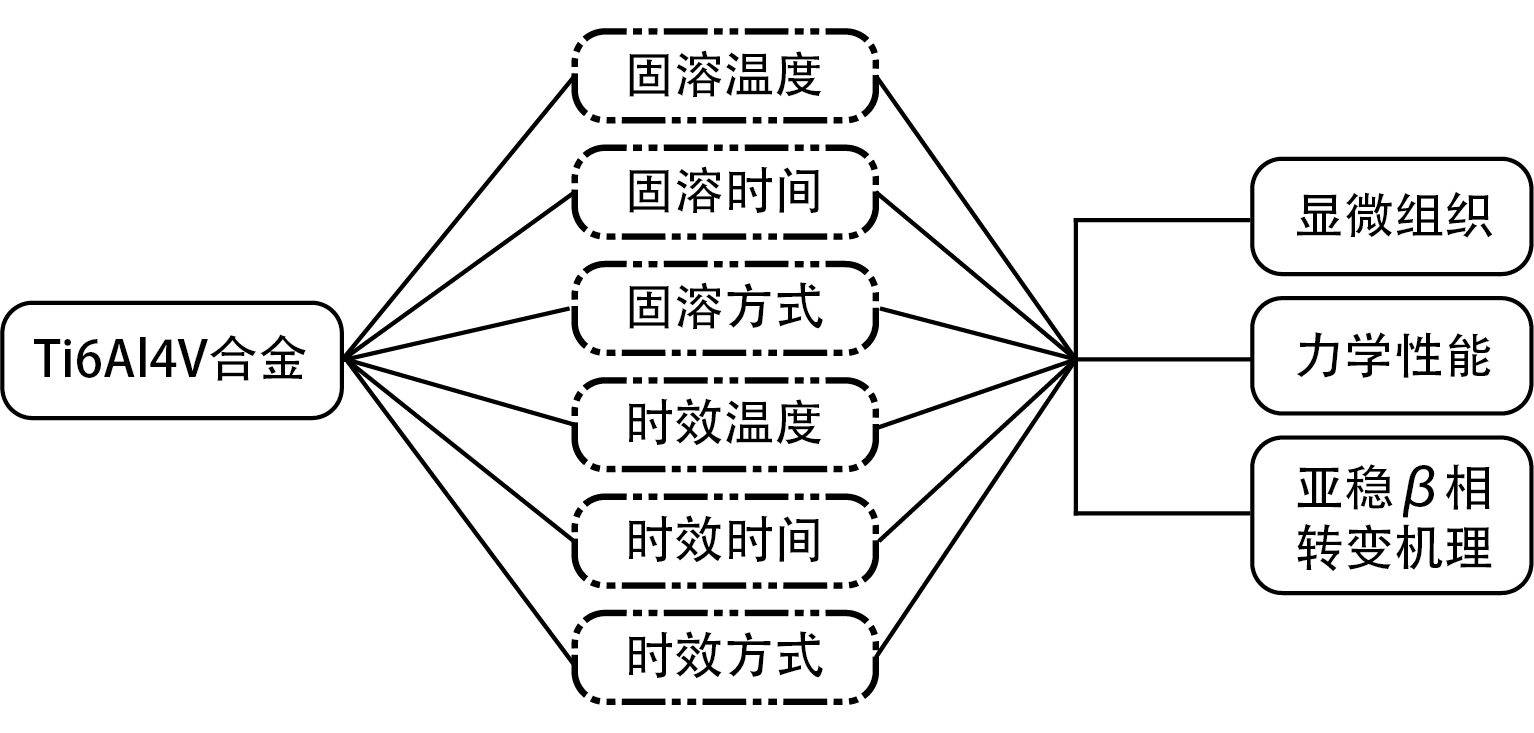
\includegraphics[width=0.7\linewidth]{pic/路线图}
	\caption{研究路线图}
	\label{fig:roadmap}
\end{figure}
